\section{Bayesian Deep Learning}
\begin{itemize}
	\item Bayesian machine learning: holding a distribution per latent variable instead of single value
	\item Benefits of Bayesian
	\begin{itemize}
		\item Ensemble modeling (better accuracies)
		\item Uncertainty estimates, preventing overconfident networks
		\item Model compression (have prior that pushes weights towards 0)
		\item \TODO{Think of more}
	\end{itemize}
\end{itemize}
\subsection{Epistemic uncertainty}
\begin{itemize}
	\item \textit{Epistemic uncertainty}: dataset limits
	\item Uncertainty that is introduced by dataset limits (unseen data $\Rightarrow$ how certain are the weights)
	\item Can be reduced by increasing the amount of data
	\item Important for safety-critical applications and small datasets
	\item Hard to model because posterior is usually intractable for complex functions like NN
	$$p(w|x,y) = \frac{p(x,y|w)p(w)}{\int p(x,y|w)p(w)dw}$$
	\item \textbf{Monte-Carlo Dropout}: apply dropout during testing (Bernoulli-distribution over weights as variational distribution). The variance/uncertainty derived from there approximates uncertainty gained by variational framework. 
	\begin{itemize}
		\item \textit{Advantages}: every standard NN can be turned into a Bayesian NN. Very easy to train and no inference network necessary
		\item \textit{Drawbacks}: expensive, have to rerun model several times on data. Not very accurate (depends on activation function etc.)
	\end{itemize}
	\item \textbf{Deep Gaussian Process}: predict mean and variance for every data point.
	\begin{itemize}
		\item The predictive distribution is $p(y|x,X,Y) = \int p(y|x,w)p(w|X,Y)dw$
		\item The likelihood term is a Gaussian $p(y|x,w)=\mathcal{N}(y; \hat{y}(x,w), \tau^{-1}I_D)$ where $\hat{y}(x,w)$ is a NN and $\tau^{-1}$ the model precision that can be derived from MC dropout
		\item For the posterior, we use variational approximation: $p(w|X,Y)\approx q(w)$. In case of MC dropout, we have $\tilde{W}_i = W_i\cdot \text{diag}\left(\left[z_{i,j}\right]_{1}^{K_i}\right), z_{i,j}\sim \text{Bernoulli}\left(p_i\right)$ where $\tilde{W}_i$ are the weights with applied dropout
		\item Minimize loss $\mathcal{L}= - \int q(w)\log p(Y|X,w)dw + KL\left(q(w)||p(w|X,Y)\right)$. First term is approximated by Monte-Carlo integration (equivalent to sampling dropout), and second can be approximated analytically
	\end{itemize}
	\item Over-paramterized models give better uncertainty estimates as they capture bigger class of models. However, they also need higher dropout rates
\end{itemize}
\subsection{Aleatoric uncertainty}
\begin{itemize}
	\item \textit{Aleatoric uncertainty}: data uncertainty
	\item Uncertainty due to the nature of data (noise/hard to predict accurate. Example: depth estimation with bad sensor)
	\item Can be reduced by better data (better sensors, multiple different sensors, etc.)
	\item \textit{Data-dependent/heteroscedastic aleatoric uncertainty}: specific raw inputs like images that are hard to interpret
	\begin{itemize}
		\item Can be modeled by predicting a variance term per data point to reduce loss
		$$\mathcal{L} = \frac{\lVert y_i - \hat{y}_i\rVert^2}{2\sigma_i^2} + \log \sigma_i$$
		If variance low, the loss is weighted higher, but the $\log$ term is smaller $\Rightarrow$ trade-off
	\end{itemize}
	\item \textit{Task-dependent/homoscedastic aleatoric uncertainty}: introduced by task like semantic segmentation or depth estimation (hard at edges). Possible solution: train on multiple tasks like edge detection
	\begin{itemize}
		\item We can as well introduce a variance term, but shared by all data points (task individual):
		$$\mathcal{L} = \frac{\lVert y_i - \hat{y}_i\rVert^2}{2\sigma^2} + \log \sigma$$
	\end{itemize}
\end{itemize}
\subsection{Bayes by Backprop}
\begin{itemize}
	\item Start from a NN with a distribution over its weights
	\item Train weights to approximate the true posterior well (similar to ELBO just with $p(\mathcal{D})=1 \Rightarrow \log p(\mathcal{D}) = 0$)
	$$\text{KL}\left(q\left(w|\theta\right)||p\left(w|\mathcal{D}\right)\right) = \text{KL}\left(q\left(w|\theta\right)||p\left(w\right)\right) - \int q(w|\theta) \log p(\mathcal{D}|w)dw$$
	First term pushes distributions towards prior, and second towards modeling the data well
	\item Compute by Monte-Carlo integration (over distribution $q(w|\theta)$) for \textit{both} terms:
	$$\mathcal{L} = \log q(w_s|\theta) - \log p(w_s) - \log p(\mathcal{D}|w_s) \hspace{2mm}\text{ where }\hspace{2mm} w_s\sim q(w_s|\theta)$$
	\item Example: assume a Gaussian variational posterior on the weights $w=\mu + \epsilon \cdot \log(1 + \exp\rho))$ (standard deviation with softplus trick for always positive values). Learn parameters $\mu$ and $\rho$ per weight
	\begin{figure}[ht!]
		\centering
		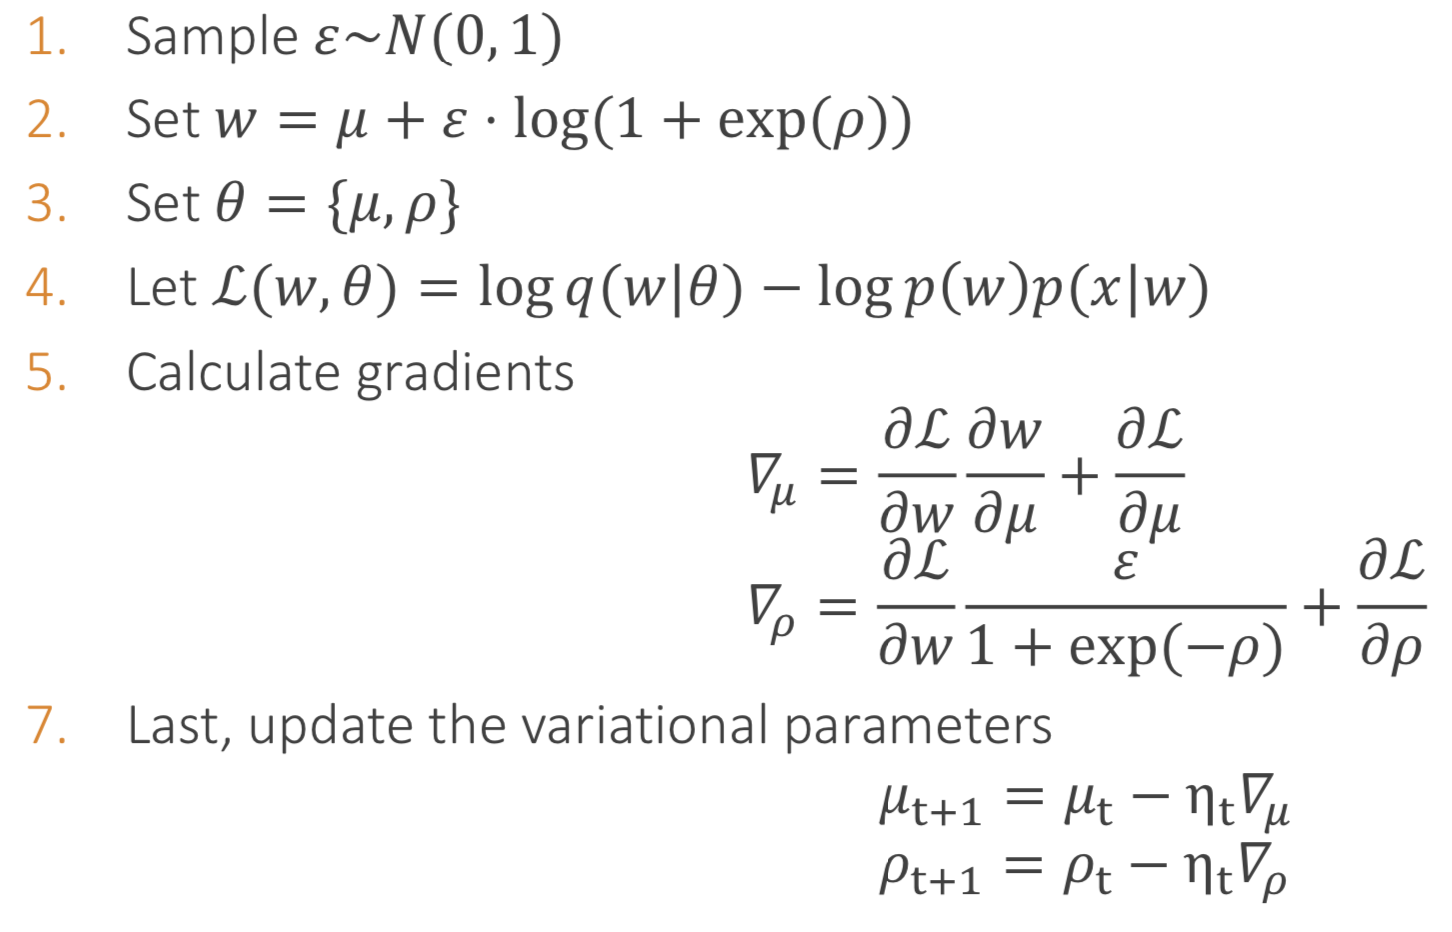
\includegraphics[width=0.4\textwidth]{figures/Bayes_By_Backprop.png}
	\end{figure}
	\item In experiments, Bayesian NNs perform similar to plain NNs with dropout
\end{itemize}